\documentclass[12pt,titlepage]{article}
\usepackage[a4paper,top=30mm,bottom=30mm,left=20mm,right=20mm]{geometry}
\usepackage{url}
\usepackage{alltt}
\usepackage{xspace}
\usepackage{times}
\usepackage{listings}
\usepackage{bbm}
\usepackage{verbatim}
\usepackage{optionman}
\usepackage{graphicx}

\newcommand{\MetagenomeThreader}{\textit{MetagenomeThreader}\xspace}
\newcommand{\GenomeTools}{\textit{GenomeTools}\xspace}
\newcommand{\nucleotide}{\textit{nucleotide}\xspace}
\newcommand{\XMLFile}{\texttt{\small{BLAST-Filename}}\xspace}
\newcommand{\MGFile}{\texttt{\small{Metagenome-Filename}}\xspace}
\newcommand{\HitFile}{\texttt{\small{Hit-Sequence-Filename}}\xspace}
\newcommand{\Gtmgth}{\texttt{gt mgth}\xspace}
\newcommand{\Gt}{\texttt{gt}\xspace}
\newcommand{\Attention}{\textbf{ATTENTION:}\xspace}

\title{\MetagenomeThreader\\
a manual}
\author{\begin{tabular}{c}
         \textit{David Schmitz-Huebsch}\\
         \textit{Stefan Kurtz}\\
         \textit{Wolfgang Streit}\\[1cm]
         Research Group for Genomeinformatics\\
         Center for Bioinformatics\\
         University of Hamburg\\
         Bundesstrasse 43\\
         20146 Hamburg\\
         Germany\\[1cm]
        \end{tabular}}
\begin{document}
\maketitle

\section{Introduction} \label{Introduction}

This document describes the \MetagenomeThreader, a software tool
for \textit{de novo} predictions of genes in sequences of metagenomeprojects.
The \MetagenomeThreader is based on the algorithem von Krause et al \cite{krause}.
For the prediction of EGTs (Environmental Gene Tags) the metagenome sequences are
blasted against a nucleotide database and the resultig BLAST-hits are used to
compute a combined score for every position in a DNA-sequence. The combinded score
reflects the potential that a specific DNA-sequence position is a coding one.

The \MetagenomeThreader is written in \texttt{C} and it is based 
on the \GenomeTools library \cite{genometools}. The \MetagenomeThreader is called
as part of the single binary named \Gt.
%The source code is single threaded and can be compiled on 32-bit and 64-bit 
%platforms without making any changes to the sources.

\section{Usage} \label{Usage}

\subsection{The meaning of used type of fonts} \label{Fonts}
Some text is highlighted by different fonts according to the following rules.

\begin{itemize}
\item \texttt{Typewriter font} is used for the names of software tools.
\item \texttt{\small{Small typewriter font}} is used for file names.
\item \begin{footnotesize}\texttt{Footnote sized typewriter font}
      \end{footnotesize} with a leading 
      \begin{footnotesize}\texttt{'-'}\end{footnotesize} 
      is used for program options.
\item \Showoptionarg{small italic font} is used for the argument(s) of an
      option.
\end{itemize}

\subsection{The functionality of the \MetagenomeThreader} \label{Functional}

The \MetagenomeThreader needs 3 data sets. It will be assumed that the metagenome
sequences are at hand. The BLAST-hits will then be generated through a BLAST of 
the metagenomesequences against a nucleotide database such as nt from NCBI.
\Attention Generating the BLAST-hits is not part of the \MetagenomeThreader and
has to be done manually. The resulting BLAST-hits have to be saved in XML-format.
If the BLAST-hits are genereated, the hit-seqeunces can be achived through the
\MetagenomeThreader. For the generation of the hit-sequence file the \MetagenomeThreader
needs a local copy of a nucleotide database, such as nt from NCBI, which will be scaned
during the \MetagenomeThreader processing. You can download a nucleotide database
from
\\
{\url{ftp://ftp.ncbi.nih.gov/blast/db/FASTA}} for example.

\subsection{The Installation of the \MetagenomeThreader} \label{Install}

The \MetagenomeThreader will be installed and is ready for use after the
installation of the \GenomeTools (see \cite{genometools} for installation instructions).
There are two different installation possibilities of the \GenomeTools in relation to the \MetagenomeThreader.
The standard installation installs the \MetagenomeThreader without the cURL-module.
If you want to install the \MetagenomeThreader including the cURL-Module you have to install the
\GenomeTools with the command \texttt{make curl="yes"}. It is only meaningful if your PC has a internet connection.
With the cURL-Module missing Hit-Sequences will be query online otherwise they
will be ignored during the computation of the EGTs.

\subsection{The Options of the \MetagenomeThreader} \label{Overview}

Since \MetagenomeThreader is part of \Gt, the \MetagenomeThreader is called as follows.

\Gtmgth $[$\emph{options}$]$ \XMLFile \MGFile \HitFile

where \XMLFile denotes the XML formatted BLAST-hit file, \MGFile the FASTA formatted
metagenomesequences file and \HitFile the FASTA formatted hit-sequences file.
The \XMLFile has to be created with a BLAST-Program. Because of the dimension of the
resulting files in metagenomeprojects a online BLAST ist not advisable or practicable.
The hit-sequence file may be empty at the first program call.
All three Files have to be given at every program call and could also be zipped files
(\texttt{\small{.gz}}).
An overview of all possible options with a short one-line descripton of 
each option is given in Table \ref{overviewOpt}.
All options can be specified only once.

\begin{table}[htbp]
\caption{Overview of the \MetagenomeThreader Options.}
\begin{footnotesize}
\[
\renewcommand{\arraystretch}{0.89}
\begin{tabular}{p{2cm}p{14cm}}\hline
\\
\Showoption{s}& specify score for a synonymic base exchange
\\
\Showoption{n}& specify score for a nonsynonymic base exchange
\\
\Showoption{b}& specify score for a blast-hit end within a query-sequence
\\
\Showoption{q}& specify score for a stop-codon within a query-sequence
\\
\Showoption{h}& specify score for a stop-codon within a hit-sequence
\\
\Showoption{l}& specify score leaving a gene on forward/reverse strand or enter a gene
on forward/reverse strand
\\
\Showoption{p}& specify maximum span between coding-regions in the same reading frame
resume as one prediction
\\
\Showoption{f}& specify maximum span between coding-regions in different reading
frames resume as coding-regions in the optimal reading-frame
\\
\Showoption{o}& specify the database name for the fcgi-database used in the cURL-module
\\
\Showoption{k}& specify the database name used for the hit-sequence extraction
\\
\Showoption{t}& specify yes$|$no if a hit-sequence file exists
\\
\Showoption{r}& specify 1$|$2$|$3 for the format of the output-file 
\\
\Showoption{a}& specify minimum length of the amino acid sequences in the result
\\
\Showoption{d}& specify minimum percent-value for species in the hit-statistic output
\\
\Showoption{e}& specify 1$|$2$|$3 for the use of alternative start-codons
\\
\Showoption{m}& specify yes$|$no if the computation should based on homology - experimental
\\
\Showoption{g}& specify yes$|$no for the \GenomeTools testmodus - output without the creating date
\\
\Showoption{x}& specify yes$|$no to extend EGTs to max length
\\
\Showoption{version}& display version information and exit
\\
\Showoption{help}& show all options
\\
\hline
\end{tabular}
%\input{ltrprogoptions}
\]
\end{footnotesize}
\label{overviewOpt}
\end{table}

%%%%
\subsection{\MetagenomeThreader Options}

\begin{Justshowoptions}

\Option{s}{\Showoptionarg{score}}{
Specify the score for synonymic base exchanges.
\Showoptionarg{score} has to be specified as a double.If this
option is not selected by the user, then \Showoptionarg{score} is set
to $1.00$ by default (recommended: positive score).
}

\Option{n}{\Showoptionarg{score}}{ 
Specify the score for nonsynonymic base exchanges. \Showoptionarg{score}
has to be specified as a double. If this option is not selected
by the user, then \Showoptionarg{score} is set to $-1.00$ by default
(recommended: negative score).
}

\Option{b}{\Showoptionarg{score}}{ 
Specify the score for a blast-hit end within a query-sequence. \Showoptionarg{score}
has to be specified as a double.
If this option is not selected by the user, then \Showoptionarg{score} 
is set to $-10.00$ by default  (recommended: negative score).
}

\Option{q}{\Showoptionarg{score}}{ 
Specify the score for a stop-codon in the query-sequence.
\Showoptionarg{score} has to be specified as a negative double.
If this option is not selected by the user, then \Showoptionarg{score} 
is set to $-2.00$ by default  (recommended: negative score).
}

\Option{h}{\Showoptionarg{score}}{ 
Specify the score for a stop-codon in the hit-sequence.
\Showoptionarg{score} has to be specified as a negative double.
If this option is not selected by the user, then \Showoptionarg{score} 
is set to $-5.00$ by default  (recommended: negative score).
}

\Option{l}{\Showoptionarg{score}}{
Specify the score for leaving a gene on forward/reverse strand or enter
a gene on forward/reverse strand. The argument \Showoptionarg{score} has to be
specified as a negative double.
If this option is not selected by the user, the default value is
set to $-2$  (recommended: negative score).
}

\Option{p}{\Showoptionarg{$S_{max}$}}{
Specify the maximum span between two coding-regions in the same reading frame
in which they resume as one coding-region.
The argument \Showoptionarg{$S_{max}$} has to be specified as a positive double.
If this option is not selected by the user, \Showoptionarg{$S_{max}$} is
set to $400.00$ by default.
}

\Option{f}{\Showoptionarg{$S_{max}$}}{
Specify the maximum span between coding-regions in different reading frames
in which they resume as coding-regions in the optimal reading-frame.
The argument \Showoptionarg{$S_{max}$} has to be specified as a positive double.
If this option is not selected by the user, \Showoptionarg{$S_{max}$} is
set to $200.00$ by default.
}

\Option{c}{\Showoptionarg{$DB_{name}$}}{
Specify the name of the database used in the cURL-Module.
The argument \Showoptionarg{$DB_{name}$} has to be chosen as a valid database
which you can find under
\\
\mbox{\url{http://eutils.ncbi.nlm.nih.gov/entrez/eutils/einfo.fcgi?}}.
If this option is not selected by the user, \Showoptionarg{$DB_{name}$} is
set to \nucleotide by default.
}

\Option{o}{\Showoptionarg{outputfilename}}{
Specify the name of the resulting outputfile where the predictions will be written to.
Each prediction will be represented by an individual block (see chapter \ref{Examples}).
If this option is not selected by the user, \Showoptionarg{outputfilename} is
set to $output$ by default.
}

\Option{k}{\Showoptionarg{$DB_{Hit-Seq}$}}{
Specify the path to the hit-sequence database.
The argument \Showoptionarg{$DB_{Hit-Seq}$} has to be chosen as a valid path to a valid
database which you can find under
\\
\mbox{\url{ftp://ftp.ncbi.nih.gov/blast/db/FASTA/}} for example.
If this option is not selected by the user, \Showoptionarg{$DB_{Hit-Seq}$} is
set to $nt.gz$ by default.
}

\Option{t}{\Showoptionarg{yes}$|$\Showoptionarg{no}}{
Specify if a hit-sequence file was already created (\Showoptionarg{yes})
or not created until now \Showoptionarg{no}. If this option is not selected by
the user, \Showoption{t} is set to \Showoptionarg{no} by default.
\Attention If there is already a hit-sequence file and you do not use \Showoption{t}
\Showoptionarg{yes} the existing hit-sequence file will be deleted.
}

\Option{r}{\Showoptionarg{1}$|$\Showoptionarg{2}$|$\Showoptionarg{3}}{
Specify the format for the output file.
You can choose between .txt (1), .html (2) und .xml (3) format.
If this option is not selected by the user, the default value of $r$
is $1$.
}

\Option{a}{\Showoptionarg{$AA_{min}$}}{
Specify the minimum number of amino-acids of the amino-acid sequences in the
output. Shorter amino-acid sequences will not appear in the output.
The argument \Showoptionarg{$AA_{min}$} has to be chosen as a value higher or equal
than 15. If this option is not selected by the user, the default value of $a$
is $15$.
}

\Option{d}{\Showoptionarg{$Stat_{min}$}}{
Specify the minimum percentage which the species must have to appear in the output-file
in the statistic section. The argument \Showoptionarg{similaritythreshold} has to
be chosen from the range [0.0,1.0] and means a percentage.
If this option is not selected by the user, the default value of $d$
is $0.0$.
}

\Option{e}{\Showoptionarg{1}$|$\Showoptionarg{2}$|$\Showoptionarg{3}}{
Specify the format for the different start-codon modes.
You can choose between (1): AUG, (2): AUG, CUG, GUG and
(3): AUG, CUG, GUG, UUG. \Showoption{e} makes only sense if \Showoption{x} is set
to \Showoptionarg{true}.
If this option is not selected by the user, the default value of $e$
is $1$.
}

\Option{m}{\Showoptionarg{yes}$|$\Showoptionarg{no}}{
Specify the computing mode. If \Showoption{m} is set to \Showoptionarg{yes},
the specified scores are used, if there are equal amino acids, otherwise they are
used if the amino acids are different. The \Showoption{m} has only experimental status.
Results are notchecked.
If this option is not selected by the user, the default value of $m$ is \Showoptionarg{no}.
}

\Option{g}{\Showoptionarg{yes}$|$\Showoptionarg{no}}{
Specify if the testmode should be use to make the results comparable in the \GenomeTools
testsuite. This option is not relevant for normal use of the \MetagenomeThreader.
If this option is not selected by the user, the default value of $g$
is \Showoptionarg{no}.
}

\Option{x}{\Showoptionarg{yes}$|$\Showoptionarg{no}}{
Specify if the extended mode should be switched on.
If \Showoption{x} is set to \Showoptionarg{yes} the computed EGTs will be extended to its max
length in both directions.
If this option is not selected by the user, the default value of $x$
is $no$.
}

\Option{help}{}{
\MetagenomeThreader will show a summary of all options on
\texttt{stdout} and terminate with exit code $0$.
}

\Option{version}{}{
Shows the version of \GenomeTools.
}

\end{Justshowoptions}

%%%%%%%%%%%%

\section{Example of a Result from the \MetagenomeThreader} \label{Examples}

\subsection{Header of the \MetagenomeThreader Result}
\label{example-results}


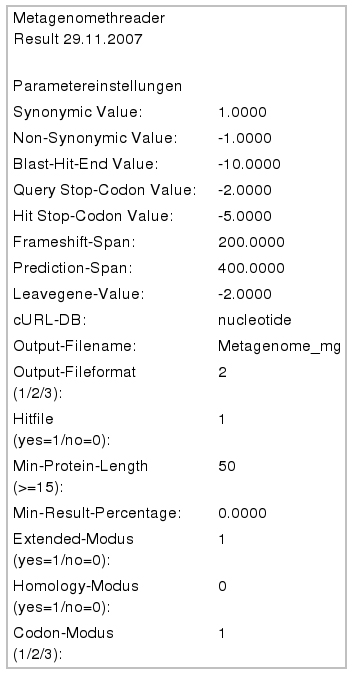
\includegraphics[height=11.51cm, width=6cm]{mgthgraphics/header_mg.jpg}

Content:
\\
- date of program execution
\\
- used program parameters

\subsection{Sequence-Section of the \MetagenomeThreader result}
\label{example-sequence}

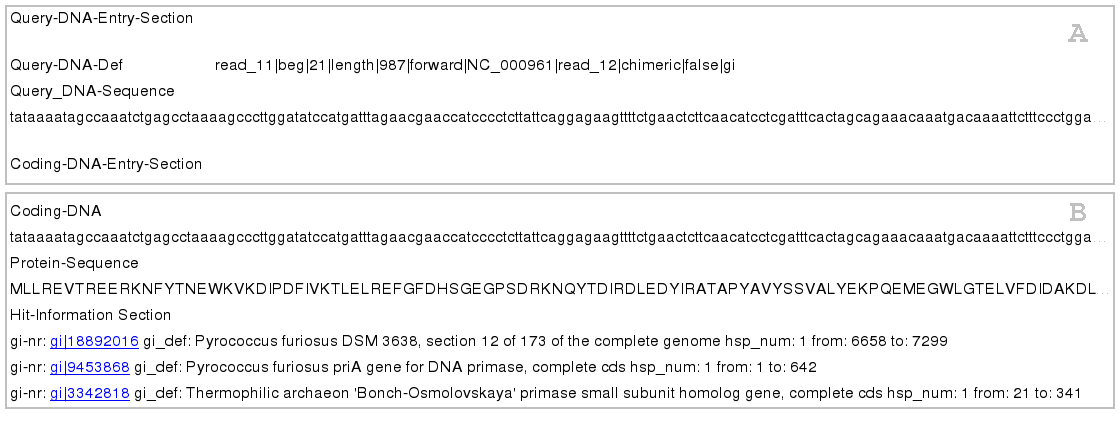
\includegraphics[height=6.02cm,width=16cm]{mgthgraphics/sequence_mg.jpg}


\begin{table}[htbp]
\renewcommand{\arraystretch}{1.0}
\begin{tabular}{p{0,3cm}p{15,7cm}}
Content:
\\
\mbox{- A:} &Output of the metagenome sequence and the metagenome sequence definition
\\
\mbox{- B:} &for every EGT
\\
&
\begin{tabular}{p{0,1cm}p{14.9cm}}
\mbox{-}& EGT DNA-sequence
\\
\mbox{-}& EGT amino acid sequence
\\
\mbox{-}& for the EGT computation used hit-definition
\end{tabular}
\end{tabular}
\end{table}

\subsection{Statistic-Section of the \MetagenomeThreader result}

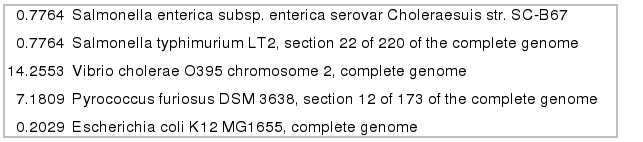
\includegraphics[height=2.64cm, width=12.01cm]{mgthgraphics/statistic_mg.jpg}

\begin{tabular}{p{0,1cm}p{14cm}}
Content:
\\
- &procentual value as the relation of the hit-sequence length
to the sequence length of all hit-sequences used for the EGT prediction
\\
- &BLAST-hit definitions
\end{tabular}

In the HTML-format the GI-number of the BLAST-hits is a hyperlink to the
linked NCBI entry.

\Attention It is recommend that you save the hit-sequence file at two
different location because if you use a existing hit-sequence file and
forget to use the -t option without the argument true the hit-sequence file
will be overwritten and you have to scan the nucleotide database and/or query
the hit-sequences online again.

%\bibliographystyle{plain}
%\bibliography{references}
\begin{thebibliography}{1}

\bibitem{krause}
L.~Krause \textit{et al}.
\newblock Finding novel genes in bacterial communities isolated
from the environment. \textit{Bioinformatics}, 22:e281-e289, 2006.

\bibitem{genometools}
G.~Gremme.
\newblock The \textsc{GenomeTools} genome analysis system.
  \url{http://genometools.org}.

\end{thebibliography}
\end{document}
